\chapter*{L'interfaccia grafica}\label{cap:interfaccia}

L'interfaccia grafica del programma permette all'utente di azionare e mettere in pausa l'accordatore e di selezionare la modalità con cui definire la frequenza di riferimento.
È possibile infatti indicare esplicitamente la nota da prendere come riferimento oppure lasciar riconoscere all'accordatore tale frequenza in modalità automatica.
Questa seconda opzione risulta comoda quando le corde della chitarra sono leggermente fuori tonalità.
In questo caso, infatti, il software riconosce facilmente la frequenza di riferimento senza la necessità che l'utente debba impostare manualmente la nuova nota di riferimento.

	\begin{figure}[h]
	  \begin{center} 
	    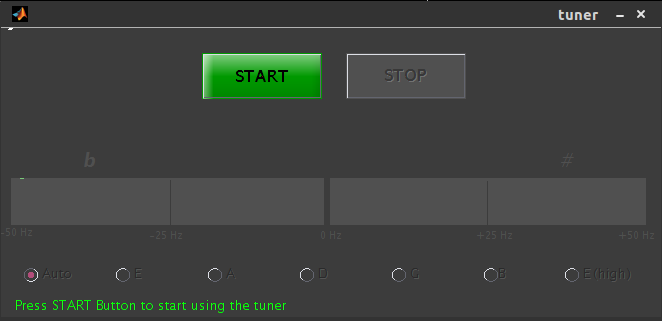
\includegraphics[width=\textwidth*\real{0.8}]{images/ch_07/accordatore_fermo.png}
	  \end{center} 
	  \caption{\textit{Accordatore pronto per essere avviato}}  
	  \label{fig:accordatore_fermo}
	\end{figure}

La figura \ref{fig:accordatore_fermo} mostra la visione che ha l'utente nel momento in cui avvia il programma.
L'accordatore è spento, per azionarlo è necessario premere il bottone \emph{Start}, come suggerisce il messaggio nell'angolo in basso a sinistra della finestra.
Al momento dell'avvio, una serie di operazioni vengono eseguite.
Innanzitutto, il bottone di start viene disattivato e il bottone di stop viene abilitato.
In secondo luogo, viene avviata la registrazione del suono dalla scheda audio e il timer che regola il funzionamento dell'accordatore si attiva.
Quest'ultimo ha la funzione di chiamare la funzione di tuning una volta al secondo. 
Tale funzione effettua le seguenti operazioni nel seguente ordine:
\begin{itemize}
	\item fermare il registratore,
	\item estrarre i dati registrati dal buffer del registratore,
	\item riattivare il registratore,
	\item chiamare la procedura di riconoscimento delle frequenza del suono in ingresso,
	\item calcolare la distanza tra frequenza del suono in input e frequenza di riferimento,
	\item aggiornare l'interfaccia grafica con i dati appena calcolati.
\end{itemize}

L'utente ha la possibilità di cambiare la frequenza di riferimento grazie ai bottoni che si trovano appena sopra il messaggio di aiuto.

	\begin{figure}[h]
	  \begin{center} 
	    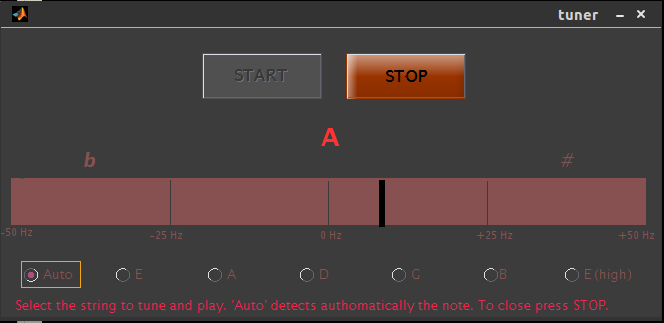
\includegraphics[width=\textwidth*\real{0.8}]{images/ch_07/accordatore_auto.png}
	  \end{center} 
	  \caption{\textit{Accordatore in funzione in modalità automatica}}  
	  \label{fig:accordatore_in_funzione}
	\end{figure}

L'aggiornamento dell'interfaccia grafica consiste nel mostrare la nota di riferimento tra i bottoni \emph{Start} e \emph{Stop} e la barra delle frequenze e la distanza misurata tra il tuono in input e quello di riferimento. 
In figura \ref{fig:accordatore_in_funzione}, la nota di riferimento è il LA (etichetta A) e la differenza risulta essere piuttosto significativa.



